% Compile twice with XeLaTeX. No shell escape or external graphics required.
\documentclass[11pt,a4paper]{article}
\usepackage[margin=21mm,headheight=15pt,headsep=8mm,footskip=11mm]{geometry}
\usepackage{fontspec}
\setmainfont{Latin Modern Roman}
\setsansfont{DejaVu Sans}
\setmonofont{DejaVu Sans Mono}[Scale=0.80]
\usepackage{unicode-math}
\setmathfont{Latin Modern Math}
\usepackage{microtype}
\usepackage{xcolor,booktabs,tabularx,array,longtable}
\usepackage{amsmath}
\usepackage{enumitem,fvextra,titlesec,fancyhdr}
\usepackage{tikz,float}
\usetikzlibrary{positioning}
\usepackage{hyperref}
\usepackage{xurl}
\definecolor{Ink}{HTML}{172C44}
\definecolor{Accent}{HTML}{087E8B}
\definecolor{Muted}{HTML}{526171}
\definecolor{Line}{HTML}{CCD8E0}
\hypersetup{colorlinks=true,linkcolor=Accent,urlcolor=Accent,citecolor=Accent,
  pdftitle={Further Lean Proof Simplifications for DiophantineConsistency},
  pdfauthor={Research and checked proof proposals},pdfsubject={New mechanisms beyond the supplied proposal corpus}}
\titleformat{\section}{\Large\sffamily\bfseries\color{Ink}}{\thesection}{0.6em}{}
\titleformat{\subsection}{\large\sffamily\bfseries\color{Ink}}{\thesubsection}{0.6em}{}
\titleformat{\subsubsection}{\normalsize\sffamily\bfseries\color{Ink}}{}{0em}{}
\titlespacing*{\section}{0pt}{3.0ex plus 1ex minus .2ex}{1.2ex}
\titlespacing*{\subsection}{0pt}{2.0ex plus .8ex minus .2ex}{.8ex}
\pagestyle{fancy}
\fancyhf{}
\fancyhead[L]{\small\sffamily\color{Muted}DiophantineConsistency / further proof simplifications}
\fancyhead[R]{\small\sffamily\color{Muted}26 October 2026}
\fancyfoot[L]{\footnotesize\sffamily\color{Muted}Pinned sources; explicit validation boundaries}
\fancyfoot[R]{\small\sffamily\thepage}
\renewcommand{\headrulewidth}{0.3pt}
\setlength{\parindent}{0pt}
\setlength{\parskip}{5.5pt plus 1pt}
\setlength{\emergencystretch}{2em}
\setlist{itemsep=2pt,topsep=4pt,leftmargin=1.5em}
\newcolumntype{Y}{>{\raggedright\arraybackslash}X}
\newcolumntype{L}[1]{>{\raggedright\arraybackslash}p{#1}}
\renewcommand{\arraystretch}{1.12}
\newcommand{\code}[1]{\texttt{\detokenize{#1}}}
\newcommand{\src}[2]{\href{https://github.com/VladimirReshetnikov/ProveIt/blob/4b3dd4efb10f1af27143a6142380322131968726/#1}{#2}}
\newcommand{\mathlibsrc}[2]{\href{https://github.com/leanprover-community/mathlib4/blob/81a5d257c8e410db227a6665ed08f64fea08e997/#1}{#2}}
\DefineVerbatimEnvironment{Lean}{Verbatim}{fontsize=\small,breaklines=true,breakanywhere=true,breaksymbolleft={},breaksymbolright={},frame=single,framesep=2.4mm,rulecolor=\color{Line},samepage=true}
\begin{document}
\thispagestyle{empty}
{\sffamily\color{Accent}\bfseries RESEARCH NOTE \quad / \quad CHECKED LEAN CANDIDATES}\par
\vspace{6mm}
{\sffamily\bfseries\color{Ink}\fontsize{29}{34}\selectfont Further Lean proof\\simplifications}\par
\vspace{3mm}
{\sffamily\Large\color{Muted}DiophantineConsistency, beyond the existing proposals}\par
\vspace{5mm}
{\large 26 October 2026}\par
\vspace{6mm}
\hrule height 0.6pt
\vspace{5mm}
\textbf{Main finding.} The strongest immediate reduction is a shared Pell ratio estimate whose error allowance is a parameter. Two long proofs become one theorem and two short wrappers. A sharper native-rank inequality removes a second mathematical duplication. Integer induction centered on the known point substantially simplifies a Wang interval argument. A bounded first-failure certificate isolates repeated minimal-index reasoning. A shared-edge representation of Wang rows is a promising structural follow-up, with a checked generic kernel and an explicit remaining integration obligation.

\textbf{Deliverable.} This note accompanies Lean examples, individual and combined patches, complete candidate source files, compiler and axiom receipts, an exclusion inventory, and portable replay scripts. The supplied patches preserve the existing public theorem statements. The recommended interval patch also preserves its exact former axiom set.

\textbf{Scope.} Source calculations and compiler checks use ProveIt commit
\begin{center}\code{4b3dd4efb10f1af27143a6142380322131968726}.\end{center}
The exclusion corpus was refreshed at commit
\begin{center}\code{23f631ea07fff8632eb8cd92286f7621bbe051c0}.\end{center}
The seven patched source files and the shared-edge proposal's target were unchanged between these commits. The later incoming proposals are reviewed separately in the accompanying freshness audit.

\textbf{How to read the evidence.} Complete candidate-module compilation, an isolated exact theorem, and a generic design kernel are different levels of evidence. They are labeled separately throughout. These checks reused dependency artifacts; they are not a clean rebuild of the entire repository. Physical line counts include helpers and wrappers where specified. They do not imply faster elaboration or a total saving relative to every possible implementation of the earlier proposals.

\vfill
{\small\color{Muted}This is a scoped non-repetition study of the supplied repository material. It makes no claim that the underlying mathematics or library APIs are new to the wider Lean literature.}
\newpage
\begingroup
\small
\setlength{\parskip}{0pt}
\tableofcontents
\endgroup
\newpage

\section{Selection rule and evidence}
\label{sec:scope}

The request is stronger than finding code that has not yet been edited: ideas already described in the research packets or incoming material must be treated as implemented. Accordingly, adoption status was ignored when deciding novelty. Deferred directions, uncompiled sketches, supplementary source notes and further-research questions all count as prior work.

The initial inventory covers all six placed packets, a--f, under \code{research/lean-proof-simplification}, their README and adoption record, and all five incoming ZIPs then present. It records 323 placed files and 400 nondirectory archive members. Of those archive members, 251 text, source, patch and metadata files were extracted for inspection; the manuscripts were read from their TeX sources. PDFs and generated files were hashed without treating old compiler outputs as evidence for the present candidates. The incoming README was searched throughout, and its relevant intake summaries were read. The initial exclusion ledger has 83 mechanisms, each linked to its supporting prior material. The supplementary freshness audit covers the four ZIPs added while this work was in progress. The final review therefore covers fifteen packets: six placed packets and nine incoming ZIPs, with 2,216 incoming nondirectory members and 2,048 extracted text/code members. Its consolidated ledger has 98 excluded mechanisms. It caused a small-square refactoring of \code{firstUnit_fundamental} to be withdrawn: the new \code{additional_lean_simplifications} packet already replaces that target by a uniform small-ordinate criterion. The withdrawn study is not included among the delivered proposals or patches.

The full audit is in \path{audit/novelty_audit.md}, with machine-readable inventories and exclusion records beside it. The method establishes non-repetition within the inspected material at the stated commits. It does not recursively claim coverage of every retired manuscript linked outside the two requested directories.

Three distinctions prevent misleading novelty claims here:
\begin{itemize}
\item Replacing artificial existential witnesses by \code{set} in the native ratio proof was already proposed. Only sharing the scale-dependent inequality is credited as new, and that older cleanup is explicitly subtracted in the ratio comparison.
\item A source-facts interface and native-rank cast conversions were already proposed. The new rank contribution is the stronger factor $2q-1$, derived from the positive transport gap. Merely placing old facts in a record, or shortening casts, contributes no new idea.
\item Generic semantic locality, scanner iteration, finite-table dispatch and controller invariants were already proposed. The Wang representation below instead makes a particular geometric matching condition structural by sharing one edge function between adjacent tile records.
\end{itemize}

\subsection{Recommendation table}

\begin{tabularx}{\textwidth}{@{}L{.21\textwidth}YL{.28\textwidth}@{}}
\toprule
\textbf{Proposal} & \textbf{Concrete payoff} & \textbf{Validation}\\
\midrule
Parameterized ratio estimate & 70 physical lines removed across two files; 66 after the explicit earlier \code{set} cleanup & Both complete changed modules; public wrappers and downstream axiom audit\\
\addlinespace[3pt]
Sharper native-rank envelope & $R\ge(2q-1)(q^2-1)$, hence $R\ge40$ and $R>3q$ & Both complete changed modules; generic 40-bound; combined arithmetic check\\
\addlinespace[3pt]
Integer induction at the seed & 26-line proof body becomes 14 lines with the old axiom footprint & Complete module and existing focused client\\
\addlinespace[3pt]
Bounded first failure & Two minimality blocks share one prefix contract; 2 net module lines saved & Complete module and existing focused client\\
\addlinespace[3pt]
Shared-edge Wang row & Horizontal matching becomes one index identity & Generic kernel checked; actual row equality and membership integration pending\\
\addlinespace[3pt]
\bottomrule
\end{tabularx}

A separate five-line trace cleanup is included as a maintenance bonus. It is not counted among the five main proposals.

\subsection{Baseline and counterfactual accounting}

The patches target a real, reproducible source snapshot. There is no single concrete tree representing all mutually optional sketches in the prior packets. Thus the conceptual baseline assumes all those ideas, while the patch and line-count baseline is the pinned code. When adopting these suggestions after the older work, place the new facts into the already established interfaces and retain only the still-needed wrappers.

This matters especially for the rank patch. The two-file total changes from 769 to 765 lines, but the four physical lines saved include a cast simplification already within the earlier proposals' scope. They should not be advertised as four novel lines saved. The new inequality is useful even if the fully refactored baseline makes its net source cost neutral. No aggregate number in the bundle is presented as a guaranteed incremental saving after every previous idea.

\section{One Pell estimate with a parameterized error allowance}
\label{sec:ratio}

\subsection{Where the duplication occurs}

\src{Computability/DiophantineConsistency/Lean/DiophantineConsistency/NativeHalfBinomial.lean}{\code{NativeHalfBinomial.lean}} contains \code{upper_estimate_scaled}. Its existing import,
\src{Computability/HilbertTenthProblem/Lean/Diophantine/Paper1980/PellRatio90.lean}{\code{PellRatio90.lean}}, contains \code{Jones1980.Ratio90.upper_estimate'}. Both declarations occupy 91 lines in the pinned source. They repeat positivity, Pell growth, perturbation and denominator-cancellation arguments. Their decisive difference is how much room is allowed for the ratio and its additive error.

Write
\[
  \xi=\frac{(U+1)^{2r}}{U^r}.
\]
The upstream proof assumes $\xi<Y+1$ and proves $c/k<\xi+1/2$. The native version assumes $\xi<2(Y+1)$ and proves $c/k<\xi+1$. The shared structure is the implication
\begin{equation}
  \kappa>0,\qquad \xi<\kappa(Y+1)
  \quad\Longrightarrow\quad
  \frac ck<\xi+\frac\kappa2.
  \label{eq:ratio}
\end{equation}
The other numerical and Pell hypotheses remain those of the existing arguments. In particular, $U,Y,r\ge1$, the sequence identities for $c,k$, $a=Y(U+1)$, $J=2r+1$, $72r<U+1$, and $16\le Y(U+1)$ are retained. Equation~\eqref{eq:ratio} is a description of the new conclusion under those hypotheses, not an unconditional numerical implication.

\subsection{Why the generalization works}

Put $\varepsilon=9/[Y(U+1)]$ and $\delta=2r\varepsilon$. The existing growth argument supplies
\[
  c\le k\xi(1+\delta), \qquad k>0.
\]
Its small-perturbation estimate gives
\[
  (Y+1)\delta<\frac12.
\]
For intuition, this last left side is
\[
  \frac{18r(Y+1)}{Y(U+1)}
  \le \frac{36r}{U+1}<\frac12,
\]
using $Y\ge1$ and $72r<U+1$. The formal argument retains the original positivity obligations and clears only positive denominators.

Since $\delta\ge0$,
\[
  \xi\delta
  \le \kappa(Y+1)\delta
  <\frac\kappa2.
\]
Combining the two displays and dividing by positive $k$ proves~\eqref{eq:ratio}. Thus the numerical scale belongs in the statement of the common theorem, while the growth and perturbation machinery is shared unchanged.

\subsection{Proposed API and migration}

The complete patch introduces \code{upper_estimate_of_ratio_envelope} in the upstream ratio module. The original upstream theorem specializes it at $\kappa=1$; the native theorem specializes it at $\kappa=2$. A compact view of the wrappers is:
\begin{Lean}
-- Upstream wrapper: original hypotheses and conclusion retained.
simpa only [one_mul] using upper_estimate_of_ratio_envelope
  hU hY hr hJ hA ha hP hc hk (κ := 1) (by norm_num)
  (by simpa only [one_mul] using hξY') h72 h16

-- Native wrapper: original hypotheses and conclusion retained.
simpa only [show (2 : ℝ) / 2 = 1 by norm_num] using
  upper_estimate_of_ratio_envelope hU hY hr hJ hA ha hP hc hk
    (κ := 2) (by norm_num) hξY' h72 h16
\end{Lean}

The upstream wrapper keeps its existing \code{hYr : U ^ r ≤ Y} argument even though the generalized core does not use it. Removing a public hypothesis merely because it becomes unused would create an unnecessary interface change. The existing downstream doubled-coordinate calculation in the native half-binomial theorem remains separate. The new scale parameter does not justify merging that step or changing its constant.

This placement uses an import edge already present in the native module. If the project prefers to avoid modifying the upstream file, an intermediate lemma module can host the generalization, but its complete source cost and dependency direction should be assessed before choosing that arrangement. The supplied candidate takes the simpler existing dependency direction.

\subsection{Measured outcome and evidence}

The upstream file grows from 472 to 484 lines; the native file shrinks from 244 to 162. The combined total is therefore 716 to 646, including the shared theorem and both wrappers. The declarations change from $91+91$ lines to $92+8+9$ lines.

The earlier incoming notes already recommend \code{set} in the analytic proof. Modeling that exact cleanup on both old copies reduces their combined starting total by four lines, to 712. Relative to this explicit counterfactual, the new factoring removes \textbf{66 lines}. This is the relevant compression claim; the separate four-line cleanup receives no new credit.

Both complete changed modules compile. Axiom reports cover the new theorem, both retained wrappers, \path{Jones1980.Ratio90.upper_estimate}\  and \code{source_half_binomial}; their lists contain only \code{propext}, \code{Classical.choice} and \code{Quot.sound}. The standalone \path{lean/RatioFactor.lean}\  checks the same mathematical mechanism under a separate namespace. Its helper name differs from the production candidate to avoid accidental ambiguity. Compiler timings in the receipts are diagnostic observations, not benchmarks.

\section{A sharper common lower envelope for the native rank}
\label{sec:rank}

\subsection{Extract the stronger mathematical fact}

Two existing proofs reconstruct the same positive transport gap and leading product:
\begin{itemize}
\item \path{source_native_rank_ge_twentyfour}\  in
\src{Computability/DiophantineConsistency/Lean/DiophantineConsistency/NativePellBootstrap.lean}{\code{NativePellBootstrap.lean}};
\item \code{source_rank_gt_three_q} in
\src{Computability/DiophantineConsistency/Lean/DiophantineConsistency/NativePellScaleBounds.lean}{\code{NativePellScaleBounds.lean}}.
\end{itemize}
Earlier proposals already cover exposing these source facts. The additional observation is that the gap proves a stronger factor than either current proof uses.

Use the source notation
\[
 q=1+x_0\beta,\quad F=x_1,\quad \alpha=x_2,\quad
 C=q-F-\alpha>0.
\]
All these inequalities are interpreted over integers, and $F,\alpha$ are positive. Consequently,
\[
  q\ge3,\qquad q-F=C+\alpha\ge2.
\]
The leading factor
\[
  G=(q-1)(q-F)+\alpha
\]
therefore satisfies
\begin{equation}
  G\ge2(q-1)+1=2q-1.
  \label{eq:G}
\end{equation}
The literal source rows identify the native rank with
\[
  R=G(q^2-1)+(M_C+M_Fq)x_0.
\]
Under the original nonnegative mask-port assumptions, the last summand is nonnegative. Equation~\eqref{eq:G} then gives the shared theorem \path{source_native_rank_envelope}\  in \code{NativePellBootstrap}:
\begin{equation}
  q\ge3\quad\text{and}\quad (2q-1)(q^2-1)\le R.
  \label{eq:rank}
\end{equation}

\subsection{Two clients of one nonlinear derivation}

For $q\ge3$, we have $q^2-1\ge8$ and $2q-1\ge5$. Hence~\eqref{eq:rank} implies
\[
  R\ge40.
\]
It also implies $R>3q$: indeed,
\[
  (2q-1)(q^2-1)\ge8(2q-1)=16q-8>3q.
\]
The old 24-bound is retained as a wrapper so existing callers remain unchanged. The scale-bound theorem also keeps its exact natural-number conclusion, converting the already obtained integer inequality at the final interface.

The crucial Lean fragment from the shared proof is:
\begin{Lean}
have hG : 2 * q - 1 ≤ (q - 1) * (q - x 1) + x 2 := by
  nlinarith [mul_nonneg (show 0 ≤ q - 1 by omega)
    (show 0 ≤ q - x 1 - 2 by omega)]
have hGL := mul_le_mul_of_nonneg_right hG
  (show 0 ≤ q ^ 2 - 1 by nlinarith)
\end{Lean}
The explicit nonnegative product supplies the nonlinear fact; the solver then combines it with the source identity. This keeps the mathematical reason for the bound visible.

\subsection{What is sharp, and what is established}

The envelope is attained by the abstract arithmetic values $q=3$, $F=1$, $\alpha=1$, $C=1$ and zero mask term, producing $G=5$ and $R=40$. This establishes sharpness for those reduced arithmetic assumptions. It does \emph{not} establish that these values extend to a solution of all the original source equations and port constraints. The bundle deliberately makes no such attainability claim.

The complete Bootstrap and ScaleBounds candidates compile, including a final check of ScaleBounds against the freshly built Bootstrap object after the compatible patches were composed. \path{lean/RankAxioms.lean}\  proves the generic implication to 40 and checks the old public endpoints. No theorem assumes consistency, an auxiliary run, or a new source certificate beyond its original hypotheses.

After the prior source-facts proposal is assumed applied, place~\eqref{eq:rank} beside those facts and make both clients consume it. The contribution is the improved inequality and shared nonlinear derivation. The physical two-file reduction of four lines is reported only as pinned-source accounting; the cast cleanup in that patch belongs to previously proposed work.

\section{Use integer induction around the known point}
\label{sec:interval}

\subsection{Choose the induction domain that matches the theorem}

The theorem \code{interval_propagate} in
\src{Computability/DiophantineConsistency/Lean/DiophantineConsistency/WangTiles942ResetRows.lean}{\code{WangTiles942ResetRows.lean}} states that a predicate known at $x_0$ propagates in both directions throughout the open interval $(l,r)$. The existing proof separately establishes $P(x_0+n)$ and $P(x_0-n)$ by natural induction, splits on the order of an arbitrary integer $x$, and reconstructs $x$ with naturalized differences.

The proof obligation is already an integer induction. Translate to $z=x-x_0$ and use the motive
\[
  l<x_0+z\;\longrightarrow\;x_0+z<r\;\longrightarrow\;P(x_0+z).
\]
The zero case is the given point. In the successor and predecessor cases, integer arithmetic transports interval membership to the preceding step. There is no need to expose two natural-difference conversions at the call site.

The recommended complete replacement is:
\begin{Lean}
have shifted (z : ℤ) : l < x₀ + z → x₀ + z < r → P (x₀ + z) := by
  induction z using Int.induction_on with
  | zero => exact fun _ _ =>
      (show P (x₀ + 0) from (by simpa only [add_zero] using h₀))
  | succ n ih =>
      intro hl hr
      simpa only [add_assoc] using
        hnext (x₀ + (n : ℤ)) (by omega) (by omega)
          (ih (by omega) (by omega))
  | pred n ih =>
      intro hl hr
      simpa only [add_sub_assoc] using
        hprev (x₀ + -(n : ℤ)) (by omega) (by omega)
          (ih (by omega) (by omega))
intro x hl hr
have he : x₀ + (x - x₀) = x := by omega
simpa only [he] using shifted (x-x₀) (by omega) (by omega)
\end{Lean}
This display is wrapped for readability; the measured candidate body occupies 14 physical source lines. The original body has 26.

\subsection{A shorter alternative and its axiom cost}

Mathlib also supplies \mathlibsrc{Mathlib/Data/Int/Init.lean\#L88-L131}{\code{Int.inductionOn'}} with an arbitrary base. It gives a nine-line proof body by choosing $x_0$ directly. Both versions preserve the exact original theorem statement and all open-interval inequalities.

There is a measurable logical difference at this version of the library. The old theorem and the translated \mathlibsrc{Mathlib/Data/Int/Init.lean\#L69-L86}{\code{Int.induction_on}} proof report exactly
\begin{center}\code{[propext, Quot.sound]}.\end{center}
The shorter \code{Int.inductionOn'} proof reports
\begin{center}\code{[propext, Classical.choice, Quot.sound]}.\end{center}
The added axiom is a standard Lean axiom, but preserving the existing footprint is a useful project constraint. The combined patch therefore uses the translated 14-line proof. The optional nine-line version is shipped independently and must not be applied on top of the recommended alternative.

Including the explicit import, the recommended complete module changes from 162 to 151 lines; the optional version would give 146. The complete recommended module and its original focused check module compile. The optional version is checked as the exact isolated theorem, not as a separate complete module build.

This remains useful after the earlier scanner refactorings: it changes the induction used for a geometric interval argument, independent of any encoded recurrence or scanner state.

\section{Return the first failure together with its valid prefix}
\label{sec:failure}

\subsection{The repeated administrative argument}

In
\src{Computability/DiophantineConsistency/Lean/DiophantineConsistency/WangTiles942InitialStrip.lean}{\code{WangTiles942InitialStrip.lean}}, both \code{left_wall_exists} and \code{right_wall_exists} choose a least index where an interior condition fails. Each proof establishes an existential witness, invokes \code{Nat.find}, gets the endpoint bound and reconstructs the valid prefix by contradiction.

The geometric arguments are asymmetric. The left proof starts at index 1, samples $T(-j)$ and uses color 2; the right proof starts at index 2, samples $T(j)$ and uses color 4. Those distinctions should remain in their respective proofs. The shared fact is only the minimality contract:
\begin{Lean}
theorem first_failure_between (P : ℕ → Prop) (lo hi : ℕ)
    (hlo : lo ≤ hi) (hfail : ¬ P hi) :
    ∃ k, (lo ≤ k ∧ ¬ P k) ∧ k ≤ hi ∧
      ∀ j, lo ≤ j → j < k → P j := by
  classical
  have hex : ∃ k, lo ≤ k ∧ ¬ P k := ⟨hi, hlo, hfail⟩
  refine ⟨Nat.find hex, Nat.find_spec hex,
    Nat.find_min' hex ⟨hlo, hfail⟩, ?_⟩
  intro j hj hlt
  exact Classical.byContradiction
    (fun hn => Nat.find_min hex hlt ⟨hj, hn⟩)
\end{Lean}

This statement returns exactly the data the caller needs: failure at $k$, an upper bound by a known failing endpoint, and the predicate at every admissible earlier point. It requires neither a monotone predicate nor a decidable predicate argument. Classical reasoning is explicit in the helper.

\subsection{Boundary cases and source impact}

If $\mathit{lo}=\mathit{hi}$, the selected point is that endpoint and the required prefix is empty. The case $\mathit{lo}=\mathit{hi}=0$ is therefore valid. A tempting helper that omits $\mathit{lo}\le j$ from the prefix statement would incorrectly demand the predicate before the allowed starting range. Keeping the lower bound explicit makes the two source applications straightforward.

The two ten-line administrative blocks become two two-line applications. The helper costs 12 lines including its documentation, and the import and spacing also count. The whole module changes from 148 to 146 lines: \textbf{two net lines}. The benefit is a common off-by-one contract and a clearer separation between least-index selection and wall classification. This is a small maintainability change, not a large compression claim.

The complete patch retains the original local conjunction shapes, so the geometric proof tails are textually unchanged. The modified module and its existing focused client compile. The standalone example proves the general helper without importing the tile language.

\section{Make Wang horizontal matching structural}
\label{sec:edges}

\subsection{A different proof view of the same row}

The current
\src{Computability/DiophantineConsistency/Lean/DiophantineConsistency/WangTiles942StepConstruction.lean}{\code{WangTiles942StepConstruction.lean}} defines \code{stepTile} by selecting a transition tile at the old head, a receiving tile at the new head and a passing tile elsewhere. Several subsequent field proofs repeat that partition. Horizontal matching is then shown by reconciling independently written west- and east-edge tests.

Instead, give the row one edge function $e:\mathbb Z\to\mathbb N$, alongside north and south functions $n,s$. Form the tile at $x$ by
\begin{equation}
  \operatorname{row}(x)=\langle e(x-1),n(x),e(x),s(x)\rangle,
  \label{eq:edge-row}
\end{equation}
using the repository's field order: west, north, east, south.

\begin{figure}[H]
\centering
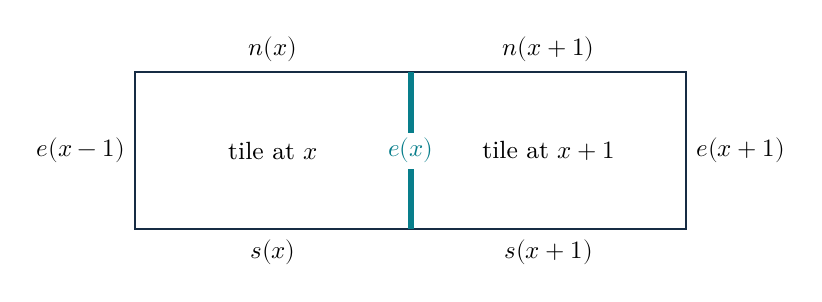
\begin{tikzpicture}[every node/.style={font=\small},line width=.7pt]
  \draw[color=Ink] (0,0) rectangle (3.5,2);
  \draw[color=Ink] (3.5,0) rectangle (7,2);
  \draw[color=Accent,line width=2pt] (3.5,0) -- (3.5,2);
  \node at (1.75,1) {tile at $x$};
  \node at (5.25,1) {tile at $x+1$};
  \node[above] at (1.75,2) {$n(x)$};
  \node[above] at (5.25,2) {$n(x+1)$};
  \node[below] at (1.75,0) {$s(x)$};
  \node[below] at (5.25,0) {$s(x+1)$};
  \node[left] at (0,1) {$e(x-1)$};
  \node[right] at (7,1) {$e(x+1)$};
  \node[fill=white,text=Accent,inner sep=2pt] at (3.5,1) {$e(x)$};
\end{tikzpicture}
\caption{The shared physical edge has one source value. Matching follows from indexing.}
\end{figure}

The horizontal theorem becomes the identity $e((x+1)-1)=e(x)$:
\begin{Lean}
theorem rowFromEdges_horizontal (north south edge : ℤ → ℕ) (x : ℤ) :
    (rowFromEdges north south edge (x + 1)).west =
      (rowFromEdges north south edge x).east := by
  exact congrArg edge (by omega)
\end{Lean}
North and south projection theorems are reflexive. This constructor alone says nothing about membership in the finite allowed tile language; that is a separate obligation.

\subsection{The machine step has one nonzero bridge edge}

Let $p$ be the old head and $d$ the actual action direction, with true meaning right. The new head is $p+1$ for a right move and $p-1$ for a left move. Define
\[
 b=\begin{cases}p&\text{right},\\p-1&\text{left},\end{cases}
 \qquad
 e(x)=\begin{cases}\rho&x=b,\\0&x\ne b,\end{cases}
\]
where $\rho$ is the actual \code{rail} value for the direction and target, including the halt target. Equivalently, $b=\min(p,\text{newHead})$.

The checked generic kernel establishes the expected edge pairs:
\begin{center}
\begin{tabular}{@{}lcc@{}}
\toprule
\textbf{Position} & \textbf{Move right: (west,east)} & \textbf{Move left: (west,east)}\\
\midrule
Old head & $(0,\rho)$ & $(\rho,0)$\\
New head & $(\rho,0)$ & $(0,\rho)$\\
Every other position & $(0,0)$ & $(0,0)$\\
\bottomrule
\end{tabular}
\end{center}
This is the real source of the current west/east case distinctions, expressed once in edge coordinates.

\subsection{Preserve the existing unconditional statements}

The actual source deliberately gives \code{stepTile_allowed} and \code{stepTile_horizontal} without a premise identifying \code{cfg.state} with the supplied state \code{q}. Only the north/south interpretation lemmas have that premise. A naive edge view using $n=\operatorname{color}(\mathit{cfg})$ would lose this distinction.

Use
\begin{Lean}
let liveCfg := { cfg with state := some q }
\end{Lean}
in the proof view. Its tape and head are unchanged, and its operating state is the supplied one. Take north colors from \code{liveCfg} and south colors from the actual machine step of \code{liveCfg}. The action and bridge are computed from the same tape bit and state as the existing construction. This makes the proposed row equality unconditional. The public north/south statements then specialize using their original premise \code{hq}.

The concrete integration should keep the executable \code{stepTile} definition and prove one equality with the edge-built view. The proof of that equality still has the three meaningful cases: old head, new head and elsewhere. It uses the existing machine color facts and the bridge-edge lemmas. Afterward, the field and matching theorems can derive from that equality. Allowedness must be preserved through the existing transition, receive and pass constructors and the real direction-specific target sets.

\subsection{Checked core and remaining experiment}

\path{lean/SharedEdgeRow.lean}\  uses a separate four-field record with the same field order as the repository tile. It checks the generic matching theorem, bridge/minimum identity and all three edge-pair cases. It intentionally does not masquerade as a complete repository refactor.

The equality with the actual \code{stepTile} and its concrete \code{Allowed} integration are \textbf{not implemented}. Until those are written, no net line saving is claimed. The experiment succeeds only if the cost of the equality and adapters is outweighed by simpler field and matching clients. The representation could still be useful for later row constructors even if the first migration is source-neutral.

This proposal neither assumes left/right symmetry of the whole tile language nor alters seam or initializer conventions. Its symmetry is limited to locating the bridge of one actual transition. That narrow scope avoids a false generalization over asymmetric seam colors.

\section{Small additional cleanup: absolute-value trace bounds}
\label{sec:trace}

In
\src{Computability/DiophantineConsistency/Lean/DiophantineConsistency/WangMachineTraceBounds.lean}{\code{WangMachineTraceBounds.lean}}, \code{run_read_of_abs_ge} converts a bound on $|x|$ to the disjunction already accepted by \code{run_read_outside}. The existing proof splits on the sign of $x$. The library equivalence supplies the conversion directly:
\begin{Lean}
exact run_read_outside M t x (le_abs'.mp hx)
\end{Lean}
The unchanged theorem checks in the complete file, and the downstream \code{halted_trace_box} axiom report remains standard-only. The six-line body becomes one line, removing five lines from the module. This is a useful local cleanup with a precise check, not a new abstract framework or evidence of a speedup.

\section{Validation, adoption and reproducibility}
\label{sec:validation}

\subsection{What was checked}

The compiler is Lean 4.32.0, release commit
\code{8c9756b28d64dab099da31a4c09229a9e6a2ef35}.
The repository pins mathlib tag \code{v4.32.0}; its manifest resolves to
\code{81a5d257c8e410db227a6665ed08f64fea08e997}.
Exact commands, candidate hashes and exit statuses accompany the bundle.

All seven proposed changed source modules were compiled in their complete form. Bootstrap was additionally compiled in the complete integrated candidate set, followed by ScaleBounds against that freshly built object. The ratio and native half-binomial modules were checked as a compatible pair. The Wang changes were checked with their original ResetRowsChecks and InitialStripChecks clients. Six unchanged small Wang support modules were compiled to supply those clients. The trace baseline and candidate were both compiled, with its BusyBeaver Core dependency compiled from pinned source.

These checks reused installed mathlib and existing project dependency objects. The broader Wang cache records origin commit \code{9bd29079d5e1c6cc1c0bcaee6cb57d59b835cba9}; the cached Language, Core, Data and DecimalMachine215 source files were individually verified byte-identical to the pinned snapshot. External BusyBeaver dependencies for that Wang closure were reused. The validation supports complete candidate-source elaboration and focused-client compatibility. It does not establish a fresh build of every dependency or all repository endpoints.

Axiom reports contain no \code{sorryAx}. The usual three axioms appear in the arithmetic and classical least-index proofs. The recommended interval theorem retains its smaller set. The checked generic shared-edge construction introduces no axiom declarations. The optional centered interval proof's extra \code{Classical.choice} is disclosed in Section~\ref{sec:interval}.

The bundle preserves a resolved initial import probe that failed because a geometry object was missing. That dependency was subsequently compiled and the focused client passed. This environmental probe is kept distinct from the successful final check results. Likewise, no isolated example is represented as proof of the unimplemented actual shared-edge adapter.

\subsection{Suggested adoption order}

\begin{enumerate}
\item Adopt the parameterized ratio theorem and its two wrappers. It gives the clearest immediate reduction and retains the existing dependency direction.
\item Add the stronger rank envelope to the already planned source-facts layer. Derive the old 24-bound and the scale-bound result from it; expose a 40-bound if a client needs that statement.
\item Apply the translated integer-induction proof. Choose the optional centered eliminator only if the slightly larger standard-axiom footprint is acceptable.
\item Adopt the least-failure helper when its prefix contract improves local readability. Its modest net source reduction does not by itself justify a large shared utility framework.
\item Trial the actual shared-edge adapter in a separate change. Measure its full definition, equality, allowedness and client cost before replacing the current proof organization.
\end{enumerate}

The combined patch includes the concrete checked changes and the trace cleanup. It excludes the generic shared-edge design and excludes the optional centered interval alternative. Individual patches allow each proposal to be assessed independently. Public theorem signatures were compared with the pinned source; byte-identical header comparisons are recorded separately.

\subsection{Replaying the bundle}

Read \path{README.md}\  and run the integrity checker before using the patches. A clean checkout at the source commit makes the line counts and source hashes reproducible. The replay script reports its plan by default; applying the patch is an explicit option. A normal dependency-resolving replay uses the repository's own Lake configuration and pinned toolchain. The provided scripts do not require the local cache paths appearing in historical receipts.

The portable scripts are syntax-checked and their integrity operations are exercised. A fresh network-dependent checkout and full clean dependency rebuild were not run as part of this report. On a later branch, apply the mathematical changes through the interfaces already adopted there, then recompile the relevant clients. The recorded source hashes make any drift visible.

Compile this report with XeLaTeX twice:
\begin{Lean}
xelatex -interaction=nonstopmode -halt-on-error report.tex
xelatex -interaction=nonstopmode -halt-on-error report.tex
\end{Lean}
No shell escape, generated image or external bibliography is needed. The report uses standard TeX packages and the Latin Modern and DejaVu fonts.

\section{Questions worth pursuing next}

The most valuable remaining experiment is the actual shared-edge equality. Does one case analysis plus field projection reduce the total size of step-row proofs, including allowedness and the state-identification adapters? The generic kernel isolates exactly what is already known and what must still be tied to the real machine.

For the rank envelope, can the full source equations force a stronger bound than 40? The present reduced arithmetic example attains 40, but it says nothing about realizability in the full source system. Any improvement must use additional genuine source constraints rather than silently assume them. Even if the constant stays 40, identifying which later estimates need only the envelope may shorten their hypotheses.

For the ratio theorem, a future caller with a different envelope $\kappa(Y+1)$ can reuse the same proof. Generalizing further should be driven by an actual client: the current $\kappa/2$ theorem already removes the observed duplication, and a more abstract perturbation interface might cost more than it saves. The exact wrappers provide a stable place to compare those choices.

For the least-failure helper, reuse should follow a matching mathematical contract. Another prefix-selection proof would justify moving the helper to a shared module. Its current local placement avoids importing machinery that the existing clients do not need.

\appendix
\section{Artifact map}

\begin{tabularx}{\textwidth}{@{}L{.34\textwidth}Y@{}}
\toprule
\textbf{Path} & \textbf{Purpose}\\
\midrule
\path{report.tex}, \path{report.pdf} & Complete narrative, mathematics, evidence and limitations\\
\addlinespace[3pt]
\path{patches/combined.patch} & Compatible concrete changes against the source pin\\
\addlinespace[3pt]
\path{patches/individual/} & Independently reviewable recommended patches\\
\addlinespace[3pt]
\path{patches/optional/} & Shorter centered interval alternative, separately checked\\
\addlinespace[3pt]
\path{candidate-source/} & Complete composed candidate source files; repository-relative paths\\
\addlinespace[3pt]
\path{lean/} & Small checked examples and public axiom audits\\
\addlinespace[3pt]
\path{evidence/} & Compiler logs, source hashes, metrics, integration and validation receipts\\
\addlinespace[3pt]
\path{audit/} & Non-repetition inventory, exclusion judgments and freshness review\\
\addlinespace[3pt]
\path{scripts/} & Portable integrity and replay utilities\\
\addlinespace[3pt]
\path{MANIFEST.sha256} & Checksums of delivered files, excluding the checksum file itself\\
\addlinespace[3pt]
\bottomrule
\end{tabularx}

Compiled dependencies and old incoming ZIPs are omitted from the deliverable. Their paths and hashes remain in the inventories. This keeps the bundle small and avoids presenting historical object files as a reproducible source environment.

\newpage
\section{Primary sources and exact targets}

All ProveIt links below are pinned to the source commit given on the title page. The freshness record supplies the later comparison and archive hashes; the \href{https://github.com/VladimirReshetnikov/ProveIt/tree/23f631ea07fff8632eb8cd92286f7621bbe051c0/docs/incoming}{final incoming exclusion snapshot} is pinned separately.
\begin{enumerate}[label={S\arabic*.}]
\item \src{Computability/DiophantineConsistency/Lean/DiophantineConsistency/NativeHalfBinomial.lean\#L18-L108}{NativeHalfBinomial, \code{upper_estimate_scaled}}, and \src{Computability/HilbertTenthProblem/Lean/Diophantine/Paper1980/PellRatio90.lean}{PellRatio90, \code{upper_estimate'}}. These are the two analytic proof sources.
\item \src{Computability/DiophantineConsistency/Lean/DiophantineConsistency/NativePellBootstrap.lean}{NativePellBootstrap}, especially \code{source_transport_positive}, \code{source_rank_eq_target} and \path{source_native_rank_ge_twentyfour}.
\item \src{Computability/DiophantineConsistency/Lean/DiophantineConsistency/NativePellScaleBounds.lean}{NativePellScaleBounds}, \code{source_rank_gt_three_q} and its natural/integer interface.
\item \src{Computability/DiophantineConsistency/Lean/DiophantineConsistency/WangTiles942ResetRows.lean\#L43-L73}{WangTiles942ResetRows, \code{interval_propagate}}.
\item \src{Computability/DiophantineConsistency/Lean/DiophantineConsistency/WangTiles942InitialStrip.lean\#L43-L119}{WangTiles942InitialStrip, left and right wall existence}.
\item \src{Computability/DiophantineConsistency/Lean/DiophantineConsistency/WangTiles942StepConstruction.lean\#L38-L148}{WangTiles942StepConstruction}, row construction, field interpretation and horizontal matching.
\item \src{Computability/DiophantineConsistency/Lean/DiophantineConsistency/WangMachineTraceBounds.lean}{WangMachineTraceBounds}, \code{run_read_of_abs_ge} and \code{halted_trace_box}.
\item \mathlibsrc{Mathlib/Data/Int/Init.lean\#L69-L131}{Mathlib integer induction principles}, at the pinned mathlib revision.
\item \src{Computability/DiophantineConsistency/research/lean-proof-simplification/README.md}{Placed simplification corpus}, \src{Computability/DiophantineConsistency/research/lean-proof-simplification/ADOPTION.md}{adoption record}, and \src{docs/incoming/README.md}{incoming index}. Exact archive-member references and digests are in the exclusion audit.
\end{enumerate}

\end{document}
